% Task 1: six signed files, one certificate that expired and was revoked, timestamps. Values from Task1/updates.json.
% CHECKED (python3, Task1/solution/check_updates.py, 2026-11-15):
%   publisher.pem: CN = Alice Software Ltd, issuer Trusty Code CA, 2024-01-01 to 2025-01-01, EKU Code Signing
%   2.1 setup: TSA time 2024-06-12; 2.2: no timestamp; 2.3: TSA time 2025-03-02;
%   2.4: the token says 2024-05-20 (edited by Mallory, the TSA signed 2025-05-20); 2.1 mirror: data changed;
%   2.2 hotfix: TSA time 2024-10-15; code-ca.crl: invalidity date 2024-09-01 (revoked 2024-09-03)
\documentclass[12pt,tikz,border=6pt]{standalone}
% Shared preamble of the task figures of Lecture 12.
% The colours and styles are copied from the preamble of ../main.tex (keep them in sync).
% Colour mapping of Lecture 12:
%   S1 indigo: Alice (signs code and mail; in HTTPS the client)   S2 pink: Mallory, a fake certificate
%   S3 violet: a certificate                  S4 amber: a private key (black text)
%   S5 teal: Bob (checks code and mail; in HTTPS owns the website)   S6 brown: a CA or a TSA
\usepackage{lmodern}
\usepackage[T1]{fontenc}
\renewcommand{\familydefault}{\sfdefault}
\usepackage{amsmath,amssymb}
\usepackage{xcolor}
\usepackage{fontawesome5}
\usetikzlibrary{arrows.meta, calc, positioning, fit, decorations.pathreplacing, backgrounds, shadows}

\definecolor{DeepBlue}{HTML}{283593}
\definecolor{AccentOrange}{HTML}{EB5A14}
\definecolor{LightGray}{HTML}{F5F6FA}
\definecolor{sIndigo}{HTML}{5C6BC0}
\definecolor{sPink}{HTML}{EC407A}
\definecolor{sViolet}{HTML}{7E57C2}
\definecolor{sAmber}{HTML}{FFB300}
\definecolor{sTeal}{HTML}{26A69A}
\definecolor{sBrown}{HTML}{8D6E63}
\definecolor{sPinkText}{HTML}{C2185B}
\definecolor{sAmberText}{HTML}{A06A00}
\definecolor{sTealText}{HTML}{00796B}
\definecolor{aExec}{HTML}{43A047}
\definecolor{aRead}{HTML}{1E88E5}
\definecolor{aWrite}{HTML}{E53935}
\definecolor{nInk}{HTML}{37474F}
\definecolor{nLine}{HTML}{90A4AE}
\definecolor{nLight}{HTML}{CFD8DC}
\definecolor{nFill}{HTML}{ECEFF1}
\definecolor{nIdle}{HTML}{E0E0E0}

\tikzset{
  hw/.style={draw=nLine, thick, fill=nFill, text=nInk, rounded corners=3pt, align=center, inner sep=4pt},
  hwmain/.style={draw=nInk, thick, fill=nInk, text=white, rounded corners=3pt, align=center, inner sep=4pt},
  container/.style={draw=nLine, thick, dashed, rounded corners=5pt},
  actor/.style={fill=#1, draw=#1, text=white, rounded corners=3pt, align=center, font=\small\bfseries, inner sep=5pt},
  actorlight/.style={fill=#1!15, draw=#1, thick, text=nInk, rounded corners=3pt, align=center, inner sep=5pt},
  person/.style={circle, fill=#1, draw=#1, text=white, minimum size=1.1cm, font=\Large, inner sep=0pt},
  data/.style={-{Stealth}, very thick, nInk},
  flow/.style={-{Stealth}, very thick, DeepBlue},
  annot/.style={draw=AccentOrange, line width=1.6pt, rounded corners=3pt},
  note/.style={font=\small, text=nInk},
  % a certificate card: violet frame, light violet fill
  cert/.style={draw=sViolet, thick, fill=sViolet!10, text=nInk, rounded corners=3pt, align=left, inner sep=5pt,
    font=\small},
  fakecert/.style={draw=sPink, thick, fill=sPink!10, text=nInk, rounded corners=3pt, align=left, inner sep=5pt,
    font=\small},
  keybox/.style={draw=sAmber, thick, fill=sAmber!25, text=black, rounded corners=3pt, align=center, inner sep=4pt},
  cabox/.style={fill=sBrown, draw=sBrown, text=white, rounded corners=3pt, align=center, font=\small\bfseries, inner sep=5pt},
  byte/.style={draw=nLine, thick, fill=white, text=nInk, font=\ttfamily\small,
    minimum width=0.72cm, minimum height=0.58cm, inner sep=1pt, rounded corners=1.5pt},
  chg/.style={byte, fill=AccentOrange!18, draw=AccentOrange, line width=1.4pt, font=\ttfamily\small\bfseries},
  rowlabel/.style={font=\small\bfseries, text=nInk, anchor=east},
}
\newcommand{\ok}{\textcolor{aExec}{\faCheck}}
\newcommand{\nok}{\textcolor{aWrite}{\faTimes}}
\newcommand{\qm}{\textcolor{AccentOrange}{\textbf{?}}}
% a file icon with a name under it: \fileicon{node name}{position}{label}
\newcommand{\fileicon}[3]{%
  \node[text=nInk, font=\fontsize{26}{28}\selectfont] (#1) at (#2) {\faFile*[regular]};
  \node[font=\scriptsize\ttfamily, text=nInk, below=0.02cm of #1] {#3};}

\begin{document}
\pagecolor{white}
\begin{tikzpicture}[>=Stealth, x=0.42cm]
  % x = months since January 2024
  \def\ty{0}
  % ---------- the time axis ----------
  \draw[nLine, very thick, -{Stealth}] (0,0) -- (37,0);
  \foreach \m/\lbl in {0/2024, 12/2025, 24/2026, 36/2027} {
    \draw[nLine, thick] (\m,-0.12) -- (\m,0.12);
    \node[font=\small, text=gray, anchor=north] at (\m,-0.15) {\lbl};
  }
  % ---------- Alice's certificate ----------
  \fill[sViolet!20, rounded corners=2pt] (0,0.35) rectangle (12,0.95);
  \draw[sViolet, thick, rounded corners=2pt] (0,0.35) rectangle (12,0.95);
  \node[font=\small, text=nInk] at (6,0.65) {\faCertificate\ Alice's certificate is valid};
  \node[font=\scriptsize, text=nInk, anchor=south] at (6,0.98) {Alice Software Ltd, code signing, 2024-01-01 to 2025-01-01};
  \draw[sViolet, thick, dashed] (12,0.35) -- (12,-9.5);
  \node[font=\scriptsize\bfseries, text=sViolet, anchor=north, fill=white, inner sep=1pt] at (12,-9.5) {expired};
  % ---------- revoked: the key is not trusted since 2024-09-01 ----------
  \draw[aWrite, thick, dashed] (8,0.3) -- (8,-9.5);
  \node[font=\scriptsize\bfseries, text=aWrite, anchor=north east, fill=white, inner sep=1pt] at (8.2,-9.5) {revoked: the key was stolen, not trusted since 2024-09-01};
  % ---------- today ----------
  \draw[AccentOrange, very thick, dashed] (34.5,1.4) -- (34.5,-9.5);
  \node[font=\small\bfseries, text=AccentOrange, anchor=south] at (34.5,1.4) {today: Bob installs};
  % ---------- the five files ----------
  \foreach \k/\f/\m/\what in {
      1/photoedit-2.1-setup.exe/5.4/{TSA stamp 2024-06-12},
      2/photoedit-2.2-update.exe/-1/{no timestamp},
      3/photoedit-2.3-update.exe/14.0/{TSA stamp 2025-03-02},
      4/photoedit-2.4-update.exe/4.6/{stamp says 2024-05-20},
      5/photoedit-2.1-setup-mirror.exe/5.4/{TSA stamp 2024-06-12},
      6/photoedit-2.2-hotfix.exe/9.5/{TSA stamp 2024-10-15}} {
    \pgfmathsetmacro{\y}{-1.45*\k}
    \node[font=\small\ttfamily, text=nInk, anchor=east] at (-0.6,\y) {\faFile*[regular]\ \f};
    \ifdim \m pt < 0pt
      \draw[nLine, thick, dashed] (0,\y) -- (34.5,\y);
      \node[font=\scriptsize, text=gray, fill=white, inner sep=1pt] at (17,\y) {signed some time, we do not know when};
    \else
      \draw[nLight, thick] (0,\y) -- (34.5,\y);
      \node[circle, fill=sBrown, text=white, inner sep=1.5pt, font=\scriptsize] at (\m,\y) {\faStamp};
      \node[font=\scriptsize, text=nInk, anchor=south, inner sep=1pt] at (\m,\y+0.2) {\what};
    \fi
    \node[circle, draw=AccentOrange, thick, fill=white, minimum size=0.7cm, font=\bfseries, text=AccentOrange] at (34.5,\y) {?};
  }
  % notes on two files
  \node[font=\scriptsize, text=sPinkText, anchor=north east] at (-0.6,-6.05) {Mallory edited the time in the token};
  \node[font=\scriptsize, text=sPinkText, anchor=north east] at (-0.6,-7.5) {a mirror site: same signature, changed bytes};
  % ---------- legend ----------
  \node[note, anchor=west, align=left] at (-14,-10.5)
    {\textcolor{sBrown}{\faStamp}\ the Time-Stamping Authority signed: ``this signature existed at this time''.\\
     Accept or reject each file today? Check the signature, the timestamp, the date and the revocation.};
\end{tikzpicture}
\end{document}
